\documentclass[12pt,twoside,a4paper]{article}
\renewcommand*\familydefault{\sfdefault}
\usepackage[utf8]{inputenc}
\usepackage[T1]{fontenc}
\usepackage[ngerman]{babel}
\usepackage[left=3cm,right=3cm,top=2cm,bottom=4cm]{geometry}
\usepackage{graphicx}
\usepackage{helvet}
\renewcommand{\familydefault}{\sfdefault}
\linespread{1.25}
\usepackage[table]{xcolor}
\usepackage{hyperref}
\hypersetup{
    colorlinks,
    linkcolor={black!},
    citecolor={blue!50!black},
    urlcolor={blue!50!black}
}
\definecolor{light-yellow}{RGB}{255, 255, 204}
\usepackage[numbib,nottoc]{tocbibind}
\usepackage{caption}
\usepackage{fancyvrb}
\usepackage{graphicx}
\usepackage{apacite}
\usepackage[acronym]{glossaries}
\makeglossaries
\newacronym{erm}{ERM}{Entity Relationship Model}
\newacronym{uml}{UML}{Unified Markup Language}
\newacronym{jakarta-ee}{Jakarta EE}{Jakarta Enterprise Edition}
\newacronym{cdi}{CDI}{Context Dependency Injection}
\newacronym{iata}{IATA}{IATA airport code}
\newacronym{ci}{CI}{Continuous Integration}
\begin{document}
\pagenumbering{gobble}
% Deckblatt
\begin{center}
\href{https://www.intension.de/}{
\includegraphics[width=6cm]{images/intension}}\hfill\href{https://www.dhbw-stuttgart.de}{
\includegraphics[width=4cm]{images/dhbw}}\\
\large
\vspace{3cm}
\textbf{Featherkraken}: Bestpreissuche für Flugangebote mit variablen Abflughäfen\\
\vspace{2cm}

\includegraphics[width=4cm]{images/featherkraken}\\
\textbf{\Large STUDIENARBEIT}
\vspace{1cm}
\\des Studienganges Informatik
\\an der Dualen Hochschule Baden-Württemberg Stuttgart
\\von
\\Ingo Kuba
\end{center}
\vspace{2cm}
\textbf{Matrikelnummer, Kurs}\hfill place, holder\\
\textbf{Ausbildungsfirma}\hfill intension GmbH\\
\textbf{Betreuer}\hfill Place Holder
\newpage
% Pre-Einleitung
\section*{Erklärung zur Eigenleistung}
Hiermit erkläre ich, dass ich die vorliegende Studienarbeit selbständig verfasst und keine anderen als die angegebenen Hilfsmittel benutzt habe.\\
Die Stellen der Studienarbeit, die anderen Quellen im Wortlaut oder dem Sinn nach entnommen wurden, sind durch Angaben der Herkunft kenntlich gemacht. Dies gilt auch für Zeichnungen, Skizzen, bildliche Darstellungen sowie für Quellen aus dem Internet.
\vspace{1cm}\\Ostfildern, den \today \hspace{1cm} \hrulefill
\newpage
% Abstract
\section*{Zusammenfassung}
% Verzeichnisse
\newpage
\tableofcontents
\newpage
\listoffigures
\newpage
\printglossary[type=\acronymtype]
\printglossary
\newpage
\interlinepenalty=10000
\pagenumbering{arabic}
\setcounter{page}{1}
% Einleitung:
\section{Einleitung}
\subsection{Motivation}
In der Regel möchte ein Fluggast den günstigsten Preis für eine bestimmte Route A nach B. Jede Flugsuchmaschine im Internet bietet diese Feature. Manchmal sucht ein Fluggast auch einfach nach Inspiration und möchte Angebote von A nach X, wobei X variabel ist. Einige Suchmaschinen bieten diese Suche bereits an. Worum es in dieser Studienarbeit geht, ist der umgekehrte Fall: X nach B. Also von welchem beliebigen Flughafen kommt man möglich günstig an ein festes Ziel.\newline
Gerade auf hochpreisigen Strecken kann es sich lohnen einen Umweg zu fliegen.
\subsection{Aufgabenstellung}
Bei der Suche sollen die klassischen Filterkriterien implementiert werden. Das heißt die Unterscheidung ob man nur einen Hinflug oder Hin- und Rückflug buchen möchte. Des weiteren soll man jeweils ein Datum für An- und Abreise festlegen können, welches um drei Tage flexibel sein soll. Neben der Buchungsklasse (Economy, Business, First Class) soll auch die Wahl der Airline oder Allianz eingeschränkt werden können. Außerdem soll man Passagier- und Umsteigeanzahl wählen können.\newline
Zusätzlich soll ein Entfernungsfilter um einen möglichen Abflughafen bereitgestellt werden. Zum Beispiel wird nur nach Angeboten gesucht, bei dem sich der Startflughafen maximal 800km (Entfernungsfilter) vom Flughafen Stuttgart (möglicher Abflughafen) entfernt befindet.\newline
Diese Flugsuchmaschine soll über ein Web-Frontend vom Nutzer bedient werden können.
\newpage
\section{Wissenschaftliche Vertiefung}
In diesem Kapitel werden technische Grundlagen aufgeführt und erläutert, welche für die Entwicklung des Projekts benötigt wurden.
\subsection{Entity Relationship Model}
Um das Datenmodell der Anwendung darzustellen wurde eine vereinfachte Variante des \acrfull{erm} verwendet.\\
\subsection*{Entities}
Ein Objekt oder Entity wird in einem Rechteck dargestellt und kann Attribute besitzen, wobei komplexe Attribute als Beziehungen zu anderen Objekten dargestellt werden. Der Name der Beziehung entspricht hierbei dem Attributnamen im Code. Die Anzahl der möglichen Relationen wird in \acrshort{uml}-Notation angegeben. Zum Beispiel ist in Abbildung \ref{fig:erm-entity} zu sehen, dass eine Person null bis n Autos besitzen kann.
\begin{center}
	\captionsetup{type=figure}
	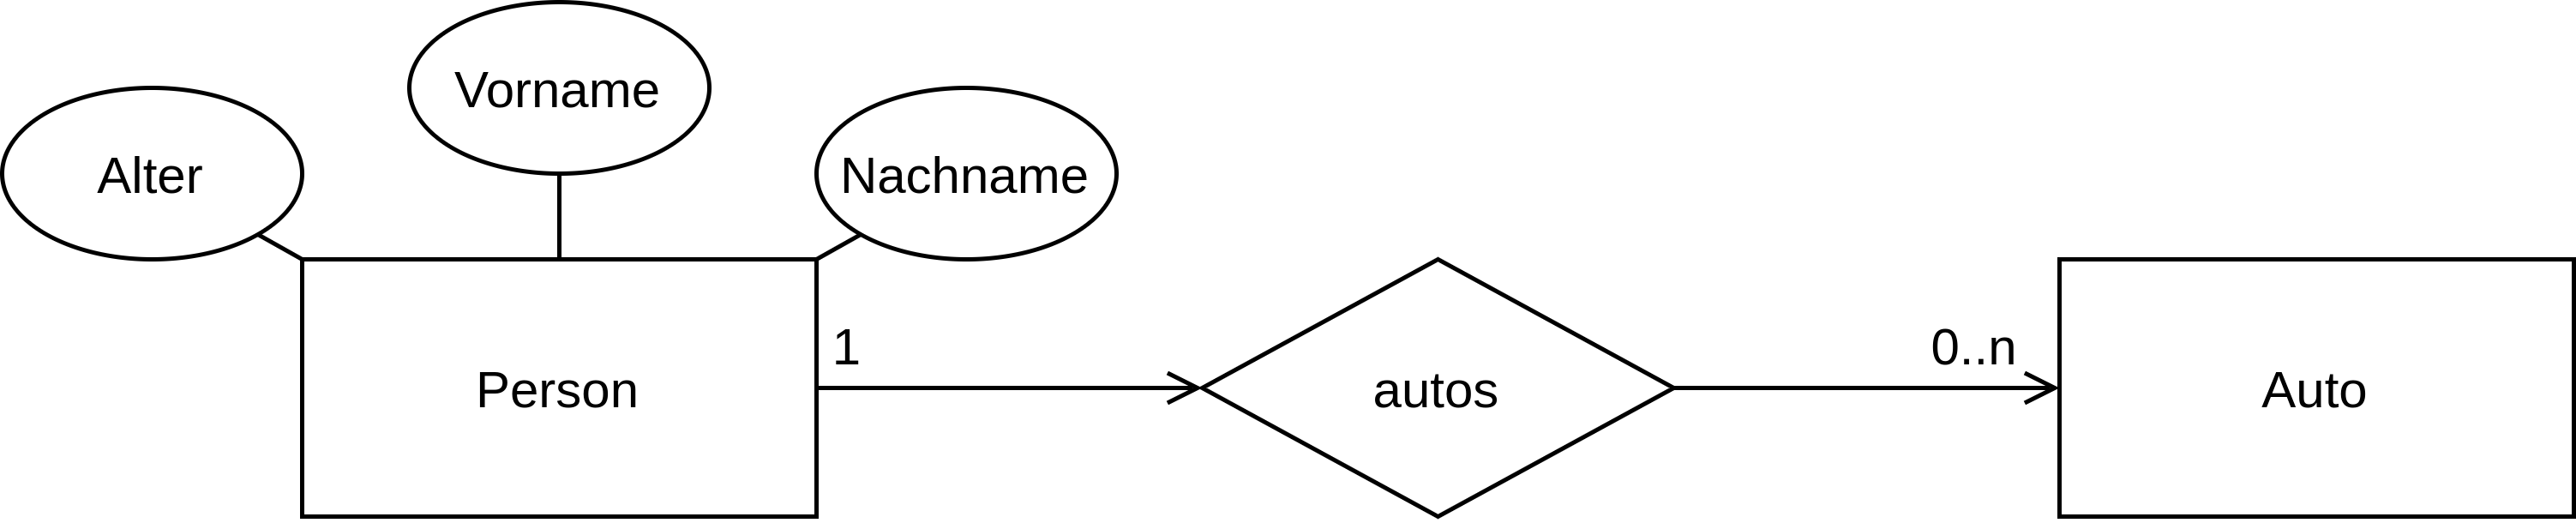
\includegraphics[width=\textwidth]{images/ERM-Entity}
	\captionof{figure}[Beispiel für eine Entity im \acrshort{erm}]{Beispiel für eine Entity mit Attributen und einer Beziehung}
	\label{fig:erm-entity}
\end{center}
\subsection*{Attribute}
Attribute können dabei eindeutig, optional oder mehrwertig sein. Die Unterscheidung zwischen Datum, Zahl oder Zeichenkette wird in einem \acrlong{erm} nicht dargestellt.
\begin{center}
	\captionsetup{type=figure}
	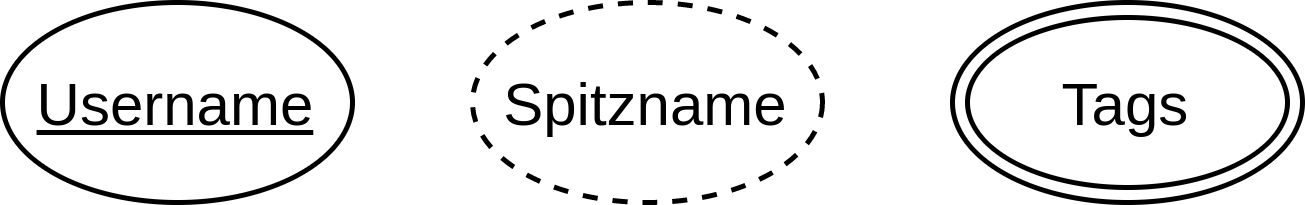
\includegraphics[width=10cm]{images/ERM-Attributes}
	\captionof{figure}[Verschiedene Arten von Attributen im \acrshort{erm}]{Attribute (v.l.): eindeutig, optional und mehrwertig}
	\label{fig:erm-attributes}
\end{center}
\subsection{Jakarta EE}\label{sec:jakarta-ee}
\acrfull{jakarta-ee} ist eine Spezifikation, welche Java SE (Standard Edition) erweitert und ermöglicht damit das Entwickeln von mehrschichtigen, zuverlässigen und sicheren Netzwerkanwendungen. Zuvor war Jakarta EE als Java EE bekannt.\newline\cite{java-ee}
\subsection{MicroProfile}\label{sec:microprofile}
Eclipse MicroProfile ist eine Erweiterung von \acrshort{jakarta-ee} und eine Alternative für Spring, welches ein Framework der Firma Pivotal ist und vielgenutzte Lösung für \acrshort{jakarta-ee} Anwendungen und Microservices.\newline
MicroProfile bietet unter anderem Unterstützung für \acrfull{cdi}, sowie eine bessere Konfigurierbarkeit der Anwendung.\newline\cite{microprofile}
\subsection{Payara}
Payara ist ein Application Server für Java-Anwendungen, insbesondere \acrshort{jakarta-ee}. Ein Application Server führt Anwendungsprogramme aus und bietet zum Beispiel Dienste für Restschnittstellen, Authentifizierung oder Datenbankzugriff. \cite{app-server}\newline
Payara basiert auf dem GlassFish Server, erweitert diesen jedoch um besseren Support sowie regelmäßigere Releases und Sicherheitsupdates.\newline\cite{payara-vs-glassfish}
\subsection{Docker}
Docker ist eine quelloffene Software zur Isolierung von Anwendungen in sogenannten Containern. Mit ihr können zum Beispiel Webserver oder Datenbanken schnell eingerichtet werden, ohne diese vorher aufsetzen zu müssen.
\subsubsection{Image}
\textit{Images} sind die Vorlage zur Erstellung neuer Container. Sie können aus mehreren Schichten von anderen Images bestehen und so können komplexe Systeme leichtgewichtig und portabel erstellt werden.
\subsubsection{Container}
Ein \textit{Container} ist die aktive Instanz eines Docker images und kann beliebig konfiguriert und bearbeitet werden. Wird ein Container beendet und ein neuer nach der Vorlage desselben Images gestartet, gehen alle Änderungen verloren. Dies lässt sich durch die Verwendung von \textit{Volumes} verhindern, welche die Konfiguration eines Containers persistieren.
\subsection{React.js}
React.js ist eine JavaScript Bibliothek um Webanwendungen zu entwickeln. Damit lassen sich einfach interaktive Oberflächen erstellen, indem man \textit{Views} für jede Komponente der Anwendung definiert. Dabei rendert React nur eine Komponente neu, wenn sich dessen Daten ändern. Dadurch wird die Anwendung effizient und der Code wird übersichtlicher und einfacher zu debuggen. Außerdem lassen sich Komponenten abstrakt definieren und mehrfach verwenden, was der gesamten Anwendung ein einheitliches Aussehen gibt. \cite{react}
\subsection{Postman}\label{sec:postman}
Postman ist ein Programm um HTTP-Schnittstellen aufzurufen. Die einzelnen Aufrufe können in sogenannten \textit{Collections} in Json-Format gespeichert werden, sodass sie in einer anderen Postman-Instanz importiert und wiederverwendet werden können. Durch diese beispielhaften Aufrufe ist es einfach, den Aufbau einer Schnittstelle zu verstehen.
\newpage
% Hauptteil
\section{Entwurf}
\subsection{Auswahl der externen API}
Um Flugdaten zu erhalten muss eine externe Schnittstelle benutzt werden, welche die Pflichtanforderungen erfüllt und dabei leicht zu verwenden ist. Die Wahl der Schnittstelle fiel dabei auf eine Rest-API, da diese sehr einfach zu benutzen sind. Für die Auswahl des Anbieters wurde eine Tabelle\textsuperscript{\ref{fig:api-comparison}} erstellt, welche die Pflichtanforderungen mit den Funktionalitäten der jeweiligen Schnittstelle abgleicht. Dabei erfüllte die API von Kiwi nicht nur alle Anforderungen, sondern war auch sehr gut dokumentiert und mit Beispielen beschrieben. Des Weiteren bot Kiwi auch eine Rest-API um Flughäfen im Umkreis gegebener Koordinaten zu finden, was der Aufgabe entgegen kam.
\begin{center}
	\captionsetup{type=figure}
	\resizebox{\textwidth}{!}
	{\begin{tabular}{ l | c | c | c | c | c | c }
		& \textbf{Skyscanner} & \textbf{Hipmunk} & \textbf{Kajak} & \textbf{Flight Data} & \textbf{Flight Bookings} & \textbf{Kiwi Flights}\\
		\hline
		\textbf{Single flight} & \cellcolor{green!50}yes & \cellcolor{green!50}yes & \cellcolor{green!50}yes & \cellcolor{green!50}yes & \cellcolor{green!50}yes & \cellcolor{green!50}yes\\
		\hline
		\textbf{Two directions} & \cellcolor{red!75}no & \cellcolor{red!75}no & \cellcolor{red!75}no & \cellcolor{green!50}yes & \cellcolor{red!75}no & \cellcolor{green!50}yes\\
		\hline
		& & & & & &\\
		\hline
		\textbf{Specific date} & \cellcolor{green!50}yes & \cellcolor{green!50}yes & \cellcolor{green!50}yes & \cellcolor{green!50}yes & \cellcolor{green!50}yes & \cellcolor{green!50}yes\\
		\hline
		\textbf{Flexible date} & \cellcolor{red!75}no & \cellcolor{yellow!75}limited & \cellcolor{yellow!75}limited & \cellcolor{green!50}yes & \cellcolor{red!75}no & \cellcolor{green!50}yes\\
		\hline
		& & & & & &\\
		\hline
		\textbf{Class} & \cellcolor{green!50}yes & \cellcolor{green!50}yes & \cellcolor{green!50}yes & \cellcolor{yellow!75}limited & \cellcolor{green!50}yes & \cellcolor{green!50}yes\\
		\hline
		\textbf{Passengers} & \cellcolor{green!50}yes & \cellcolor{green!50}yes & \cellcolor{green!50}yes & \cellcolor{red!75}no & \cellcolor{green!50}yes & \cellcolor{green!50}yes\\
		\hline
		\textbf{Airline} & \cellcolor{green!50}yes & \cellcolor{red!75}no & \cellcolor{red!75}no & \cellcolor{red!75}no & \cellcolor{red!75}no & \cellcolor{green!50}yes\\
		\hline
		\textbf{Stops} & \cellcolor{red!75}no & \cellcolor{red!75}no & \cellcolor{red!75}no & \cellcolor{red!75}no & \cellcolor{red!75}no & \cellcolor{green!50}yes
	\end{tabular}}
	\captionof{figure}[Vergleich der APIs]{Tabelle zum Vergleich der APIs}
	\label{fig:api-comparison}
\end{center}
\newpage
\subsection{Datenmodell}
Das \acrlong{erm} für das Datenmodell wurde hier aufgeteilt in Suchanfrage (\texttt{SearchRequest}) und Suchergebnis (\texttt{SearchResult}).
\subsubsection{SearchRequest}
Eingehende Anfragen an den Service (\texttt{SearchRequest}) haben verschiedene Parameter, welche die zuvor genannten Pflichtanforderungen abdecken. Komplexe Attribute wie die Zeitspanne (\texttt{Timespan}) für An- und Abreise sowie den Ursprungs- und Ziel-Flughafen (\texttt{Airport}) wurden in eigene Objekte ausgelagert, damit sie so wiederverwendet werden können.
\begin{center}
	\captionsetup{type=figure}
	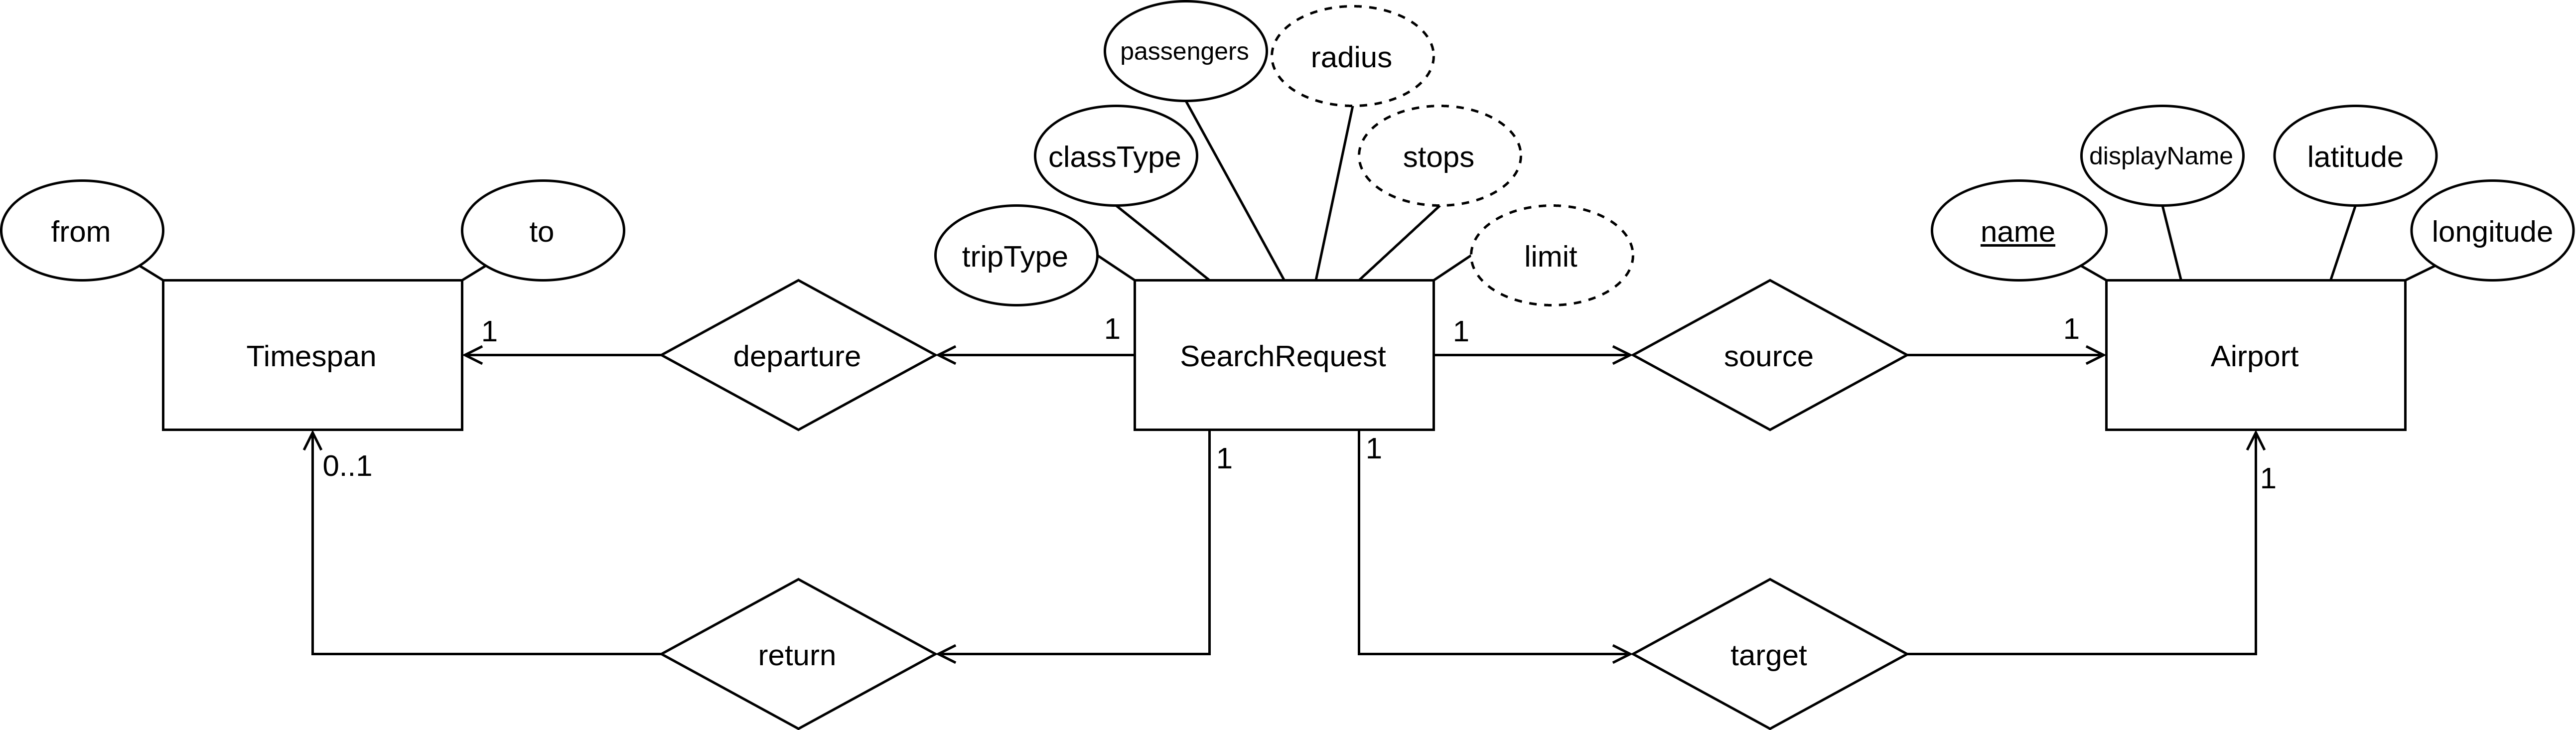
\includegraphics[width=\textwidth]{images/datamodel-SearchRequest}
	\captionof{figure}[\acrshort{erm} SearchRequest]{\acrlong{erm} des SearchRequest Objekts}
\end{center}
\subsubsection{SearchResult}
Antworten des Service (\texttt{SearchResult}) sind etwas komplexer als Anfragen aufgebaut, teilen jedoch manche Attribute beziehungsweise Objekte mit diesen. So enthält ein Suchergebnis eine Ansammlung von sogenannten \texttt{Trips}, welche sich aus Flügen (\texttt{Flight}) der An- und Abreise zusammensetzen. Diese Flügen haben widerrum selbstverständlich selbst jeweils einen Start- und Zielflughafen, welche in dem \texttt{Route}-Objekt mit Informationen zu Abflug- und Ankunftzeiten sowie der Airline enthalten sind.\\
Bei erster Betrachtung fällt auf, dass Informationen über Airlines und Zeiten redundant sind, was jedoch für die optimale Anzeige in der Oberfläche gedacht ist.
\begin{center}
	\captionsetup{type=figure}
	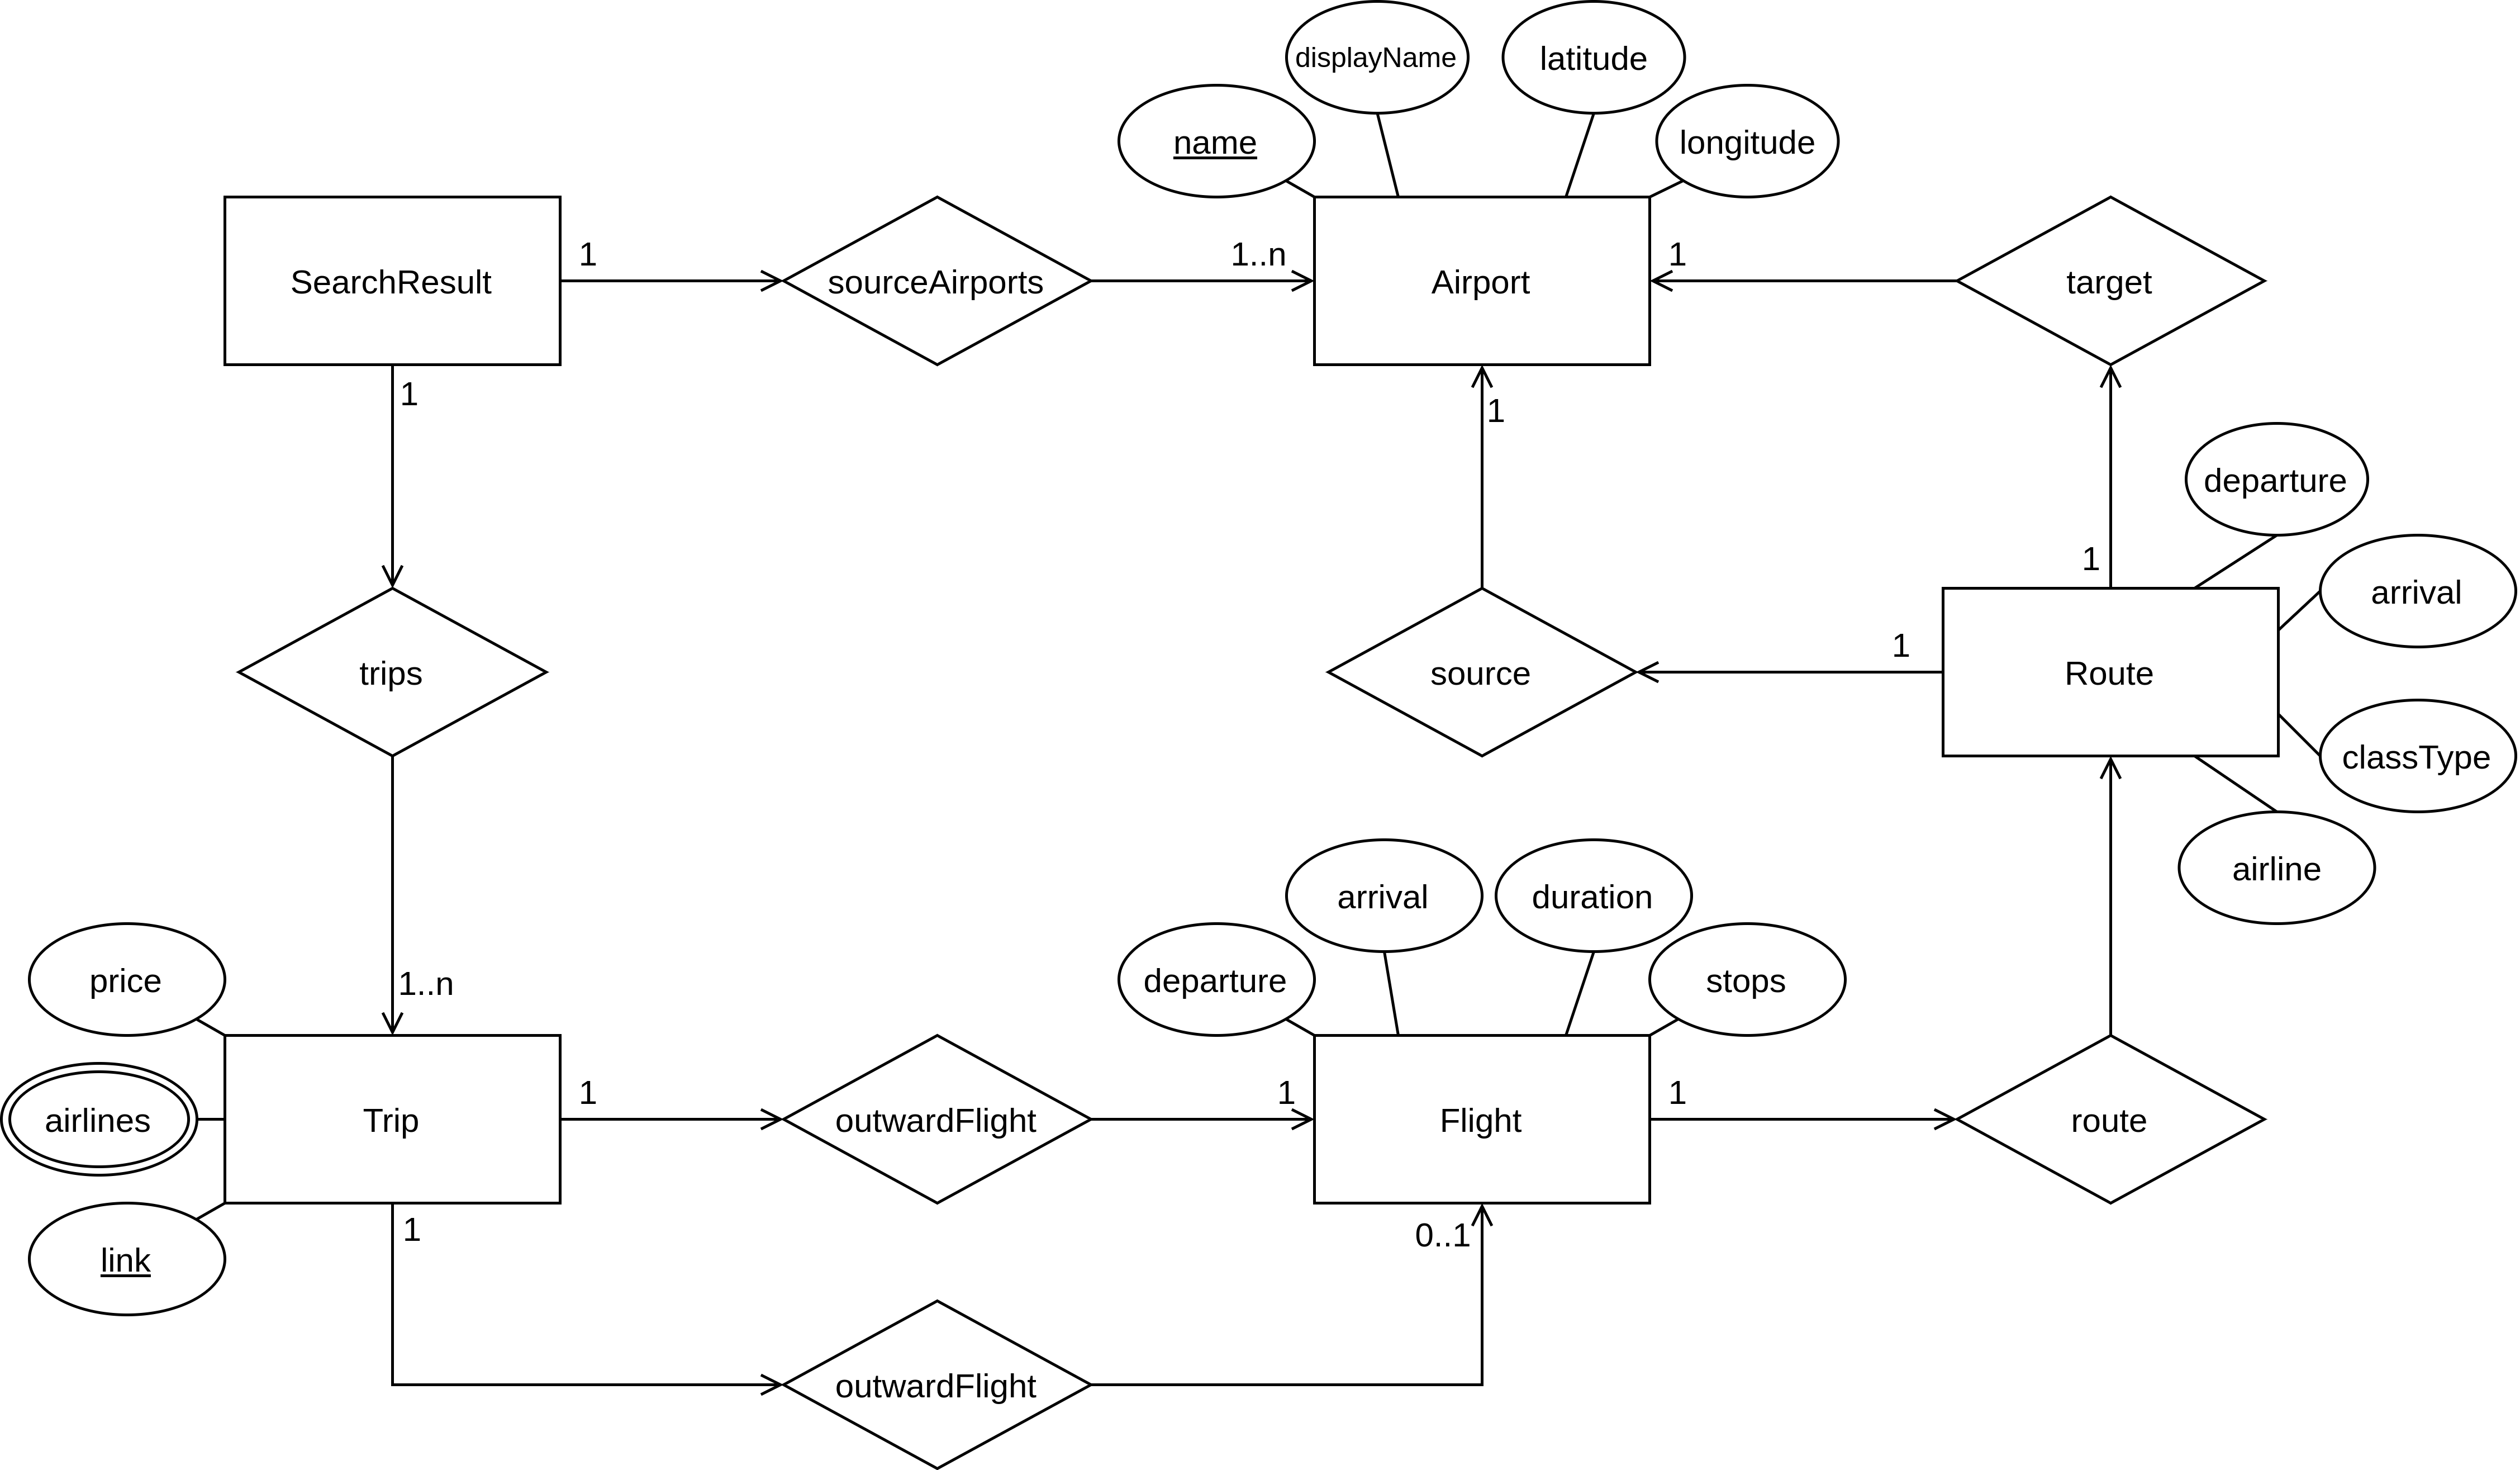
\includegraphics[width=\textwidth]{images/datamodel-SearchResult}
	\captionof{figure}[\acrshort{erm} SearchResult]{\acrlong{erm} des SearchResult Objekts}
\end{center}
\newpage
\subsection{Framework}
Die Anwendung wird in eine Server- und eine Web-Anwendung unterteilt, für welche jeweils eine Framework-Technologie gewählt werden muss. Die Serveranwendung übersetzt Suchanfragen von der Oberfläche zu einem Format, welches die externe Schnittstelle akzeptiert und leitet das Sucherergebnis daraufhin an die Oberfläche zurück. Dies bedeutet, dass die Serveranwendung als Rest-Client für die externe Schnittstelle und selbst als Rest-Schnittstelle für die Oberfläche dient.\\
Für die Komponenten war das Thema Plattformunabhängigkeit sehr wichtig und aus eigener Erfahrung eignet sich dafür Java sehr gut, da es eine große Community hat und eine Anwendung in kurzer Zeit aufgesetzt ist. Außerdem bietet Java einfache Möglichkeiten eine externe Rest-Schnittstelle anzusprechen.\\
Als Bedingung für die Web-Oberfläche ist es unabdingbar, dass die Anwendung intuitiv bedienbar ist und auf allen Endgeräten gut dargestellt werden kann. Für diesen Zweck kommen eigentlich nur drei Frameworks in Frage: Angular, React.js und Vue.js. Dabei wurde React gewählt, welches sich besser als Vue.js und Angular für kleine Anwendungen eignet, wie es in diesem Fall zutrifft. Bei dem hier vorliegenden Fall wird es sogar eine sogenannte Single-Page-Webapplication, das heißt die gesamte Funktion kann auf einer Seite dargestellt werden.
% Umsetzung
\section{Implementierung}
\subsection{Backend}
Das Backend der Anwendung dient als Proxy zwischen Web-Frontend und externer API und wurde in Java geschrieben. Dabei wurde Jakarta EE\textsuperscript{\ref{sec:jakarta-ee}} und Eclipse Microprofile\textsuperscript{\ref{sec:microprofile}} verwendet, um eine Rest-Schnittstelle für die Suche von Flügen zu bieten. Durch das Verwenden von Microprofile lässt sich die Anwendung einfach in einem Payara Application Server starten. Dieser wurde mithilfe eines Docker Images umgesetzt und dadurch lässt er sich einfach in einer Cloud Umgebung oder klassisch auf einem Windows- oder Linux-Server deployen.
\begin{center}
	\captionsetup{type=figure}
	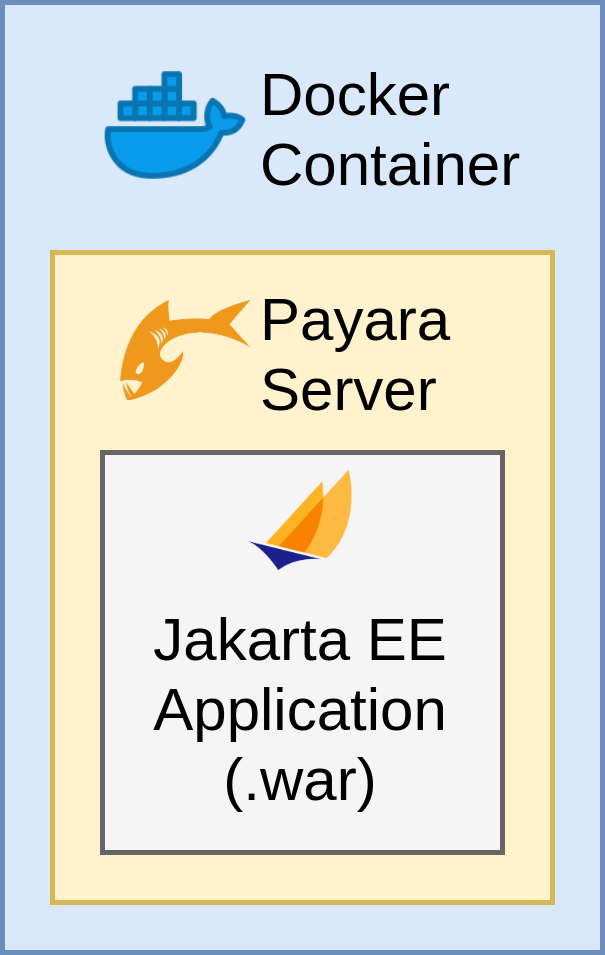
\includegraphics[height=5cm]{images/backend-structure}
	\captionof{figure}{Aufbau des Backends}
\end{center}
\subsubsection[Flughafensuche]{Flughafensuche: GET /airports}
Um bestimmte Flughäfen mit einem Teil des Namens des Flughafens oder der Stadt suchen zu können, gibt es den Endpoint \texttt{/airports} der mit einem GET-Request erreicht werden kann. Die Eingabe wird über den Query-Parameter 'query' in der URL des Requests übergeben. Ein beispielhafter Request für die Suche von Flughäfen in Amsterdam kann zum Beispiel folgendermaßen aufgebaut sein:\\
\begin{center}
	\texttt{GET www.featherkraken-example.com/airports?query=Ams}
\end{center}
Damit werden alle Flughäfen gesucht, welche den Wortteil 'Ams' im \acrlong{iata} oder Städtenamen enthalten. Die Antwort des Services besteht aus einer Liste aus gefundenen Flughäfen, welche jeweils \acrlong{iata}, vollen Anzeigenamen und Koordinaten enthalten.
\subsubsection[Flugsuche]{Flugsuche: POST /flights}
Die Kernfunktion der Anwendung steckt hinter dem Endpoint \texttt{/flights}, welcher eingehende Suchanfragen in ein für die externe API verständliches Format übersetzt und das Suchergebnis dann zurückgibt. Suchparameter werden hier nicht in der URL des Requests übergeben, sondern mit einem POST im Request-Body, da die Suchanfrage so übersichtlicher und leichter zu dokumentieren ist. Bei der Suche kann wahlweise ein Radius angegeben werden, dann werden Flüge von umliegenden Abflughäfen gesucht. So kann eine Suchanfrage für Flüge von Frankfurt und Umgebung (100km) zum Beispiel so aussehen:\\
\begin{Verbatim}
{
	"source": {
		"name": "FRA",
		"displayName": "Frankfurt International Airport",
		"latitude": 50.033056,
		"longitude": 8.570556
	},
	"target": {
		"name": "LAX",
		"displayName": "Los Angeles International",
		"latitude": 33.9425,
		"longitude": -118.40806
	},
	"radius": 100,
	"passengers": 1,
	"departure": {
		"from": "11.11.2020"
		"to": "13.11.2020"
	},
	"return": {
		"from": "22.11.2020"
	},
	"classType": "Economy",
	"tripType": "Round trip"
}
\end{Verbatim}
Für die Flughafenobjekte in \texttt{source} und \texttt{target} ist nur der eindeutige \acrlong{iata} in \texttt{source.name} entscheidend. Der Radius wird in Kilometern angegeben. In diesem Beispiel werden Hin- und Rückflüge zwischen Frankfurt und Los Angeles in der Klasse 'Economy' gesucht. Außerdem ist zu erkennen, wie ein variables Abflugdatum (11.11. - 13.11.2020) angegeben werden kann.
\section{Testing}
Das Testen der Anwendung war ein wichtiger Teil für den Erfolg des Projekts. Deshalb wurden nicht nur alle Software-Komponenten mit Unit-Tests abgedeckt, sondern auch Integrations-Tests geschrieben. All diese Tests werden programmatisch ausgeführt und werden von einer \acrshort{ci} in GitHub automatisch bei jedem \textit{push} ausgeführt. Ein \textit{merge} in den Master ist nur möglich wenn alle Tests erfolgreich ausgeführt wurden. Für alle Testfälle wurden realitätsnahe Bedingungen und Daten gewählt.\\
Des Weiteren wurde die Oberfläche, und somit das gesamte System mit der Erwartung der gewünschten Ergebnisse manuell getestet und abgeglichen.
\subsection{Automatische Tests}
Das Java-Backend wurde mit Unit- und Integrationstests getestet, welche mit dem Testframework JUnit 5 geschrieben wurden. Dadurch fallen neue Bugs schon direkt bei der Entwicklung auf. Des Weiteren wird die Qualität des Codes mit \textit{Sonar} überprüft. Dazu zählen unter anderem Aspekte wie Bugs, Schwachstellen (\textit{Vulnerabilities}) oder Verletzung von Java-Richtlinien (sogenannte \textit{Code Smells}). Um Schwachstellen in externen Bibliotheken der Anwendung aufzudecken wird \textit{OWASP} verwendet.\\
All diese Tests werden automatisch in der \acrfull{ci} von \textit{CircleCI} ausgeführt, wenn die Änderungen in das GitHub Repository gepusht werden. Pull Requests sind so konfiguriert, dass sie nur nach erfolgreichem Durchlauf der Tests akzeptiert werden können. Außerdem wird die Testabdeckung bei jedem Durchlauf dokumentiert und überprüft und darf niemals abnehmen. Die Konfiguration dieser Überprüfungen kann dem Dokument \href{https://github.com/featherkraken/featherkraken/blob/master/.circleci/config.yml}{\texttt{featherkraken/.circleci/config.yml}} entnommen werden.\\
Die Komponenten des React-Frontends wurden aus Zeitgründen nicht mit automatischen Tests abgedeckt, jedoch wird die Kompilierbarkeit der Anwendung in \textit{CircleCI} überprüft und der Stand des \textit{master}-Branches in GitHub Pages automatisch veröffentlicht. Dies kann in \href{https://github.com/featherkraken/featherkraken-ui/blob/master/.circleci/config.yml}{\texttt{featherkraken-ui/.circleci/config.yml}} eingesehen werden.
\subsection{Manuelle Tests}
Zusätzlich zu den automatischen Tests gibt es eine \textit{Postman-Collection}\textsuperscript{\ref{sec:postman}} für die Rest-Schnittstellen des Backends. Diese kann unter \href{https://github.com/featherkraken/featherkraken/blob/master/src/test/postman/Collection.json}{\texttt{src/test/postman/Collection.json}} gefunden und in \textit{Postman} importiert werden.\\
Außerdem gibt es Testfälle für das Frontend, um die Umsetzung der Anwendung mit den tatsächlichen Anforderungen vergleichen zu können:
\begin{center}
	\captionsetup{type=figure}
	\resizebox{\textwidth}{!}
	{\begin{tabular}{ l | l | l | l }
			\textbf{Abflughafen} & \textbf{Zielflughafen} & \textbf{Klasse} & \textbf{Erwartung} \\
			\hline
			Inverness INV & John F. Kennedy International JFK & First class &  Umstieg mit Economy Klasse wird gefunden\\
			\hline
			Heathrow LHR & John F. Kennedy International JFK & First class &  Flüge werden gefunden\\
			\hline
			Munich MUC (+600km) & Kyiv International Airport (Zhuliany) IEV & Economy &  Flug von LEJ gefunden\\
			\hline
			Stockholm Arlanda ARN & Dubai International DXB & First class &  Umstieg mit Business Klasse wird gefunden\\
			\hline
			Sofia SOF & San Francisco International & Business &  Umstieg mit Economy wird gefunden\\
	\end{tabular}}
	\captionof{figure}[Testfälle des Frontends]{Tabelle für die Testfälle des Frontends}
	\label{fig:ui-tests}
\end{center}
\newpage
% Ende
\section{Fazit}
Zunächst wird hier in einem Ausblick auf Möglichkeiten zur Verbesserung der Anwendung eingegangen, denn Software-Entwicklung ist ein niemals abgeschlossener Vorgang. Danach werden bekannte Probleme und Einschränkungen aufgelistet, die noch nicht gelöst werden konnten, jedoch wird ein Lösungsansatz zum weiteren Vorgehen aufgeführt. Alle Probleme sind in GitHub Issues festgehalten, sodass sie nicht in Vergessenheit geraten können. Zum Abschluss wird das gesamte Projekt noch einmal zusammengefasst.
\subsection{Ausblick}
Um die Funktion der Anwendung zu erweitern könnte man zum Beispiel weitere externe Schnittstellen anbinden, um eventuell billigere Flüge als die von Kiwi.com zu finden. Dazu wurden die betroffenen Klassen des Java-Backends schon so abstrakt geschrieben, sodass dies mit angemessenen Aufwand umsetzbar ist.\\
Dabei ist jedoch anzumerken, dass diese externen Aufrufe bist jetzt nicht asynchron erfolgen. Das heißt dass gewartet wird, bis alle externen APIs geantwortet haben. Das hat zur Folge, dass die Antwortzeit äquivalent zur langsamsten externen API ist. Um das zu ändern, muss evaluiert werden, ob Rest-Calls asynchron beantwortet werden können.\\
Außerdem kann die Geschwindigkeit der Aufrufe dokumentiert werden. Damit kann entschieden werden, ob bestimmte externe APIs zu langsam sind und damit wieder entfernt werden sollten. Für diese Art von Monitoring gibt es bereits Lösungen wie \href{https://prometheus.io/}{\textit{Prometheus}} oder die eingebaute Funktion von Eclipse Microprofile mithilfe sogenannter \textit{Metrics}.\\
Des Weiteren kann auch ein Entfernungsfilter für den Zielflughafen auf die selbe Art wie für den Startflughafen hinzugefügt werden. Dazu müsste das Backend und die Oberfläche angepasst werden. Da dies jedoch nicht im Fokus der Aufgabe stand, sei dies hier jedoch nur als Idee anzumerken.\\
Bei der Entwicklung der Anwendung fiel außerdem auf, dass es neben der Rest-Schnittstelle von Kiwi.com eine äquivalente GraphQL-Schnittstelle gibt. Das könnte bedeuten, dass die Rest-Schnittstelle veraltet ist und deshalb bestimmte Probleme auftreten (siehe \ref{sec:mixed-classes}). In diesem Fall wäre es ratsam, auf die GraphQL-Schnittstelle umzusteigen.\newline\cite{kiwi-tequila}
\subsection{Bekannte Probleme}
\subsubsection{AirportsFinder}
Die externe Schnittstelle \href{https://rapidapi.com/cometari/api/airportsfinder}{AirportsFinder} zur Suche von Flughäfen in einem bestimmten Radius scheint eine Priorisierung der Flughäfen oder eine Einschränkung der Ergebnismenge vorzunehmen. So kann man zum Beispiel den Flughafen 'Leipzig/Halle LEJ' von Berlin aus mit einem Radius von 150km finden, jedoch nicht von München mit einem Radius von 360km. Dies hat zur Folge, dass für manche Flüge nicht der absolut günstigste Flug gefunden werden kann. Deshalb muss in Zukunft eine andere externe Schnittstelle zum Suchen von Flughäfen in einem gegebenen Radius gefunden werden.
\subsubsection{Suche mit gemischten Klassen}\label{sec:mixed-classes}
Die externe API für die Flugsuche bietet die Möglichkeit, mit dem Parameter \texttt{mix\_with\_cabins} über mehrere Klassen zu suchen, wenn keine Flüge in der angegebenen Klasse gefunden werden können. Diese Funktion ist bei der API von Kiwi.com nicht gut dokumentiert oder fehlerhaft umgesetzt. Zur Lösung für dieses Problem könnten weitere Anfragen mit anderen Klassen abgeschickt werden, wenn die gegebene Klasse keine Ergebnisse liefert.
\subsubsection{Deployment des Backend}
Es wurde versucht die Java-Anwendung auf \textit{Heroku} zu hosten, damit sie jederzeit im Internet genutzt werden kann. Dies war aber selbst nach vielen Tagen nicht nachvollziehbar, also wurde dieser Ansatz verworfen. Als Zwischenlösung könnte die Anwendung auf einem Linux-Server bereitgestellt werden. Dies sollte automatisch mit jeder Änderung im GitHub Repository erfolgen, wie es mit \textit{Heroku} versucht wurde.
\subsubsection{Sortieren/Filtern der Suchergebnisse}
Das Sortieren oder Filtern der Suchergebnisse - zum Beispiel nach Abflughafen oder Airline - stellte sich komplizierter als gedacht heraus. Leider konnte dazu kein Experte in React.js oder TypeScript gefunden werden. Wenn sich einer finden lässt, ist dieses Problem in angemessener Zeit zu lösen.
\subsection{Zusammenfassung}
% Literaturverzeichnis
\newpage
% set interlinepenalty to not split entries on page break
\bibliographystyle{apacite}
\bibliography{paper}
\end{document}